\section{RANSOM: System Design and Implementation}
In light of the results presented in the previous section, we see that an 
overlay network can significantly help a client avoid any given country.  
Therefore, we have designed and developed a system, RANSOM, that allows users 
to route around a specified country.

\subsection{Architecture}

There are three main components to RANSOM: the oracle, the relays, and the 
clients.  Figure \ref{fig:arch} shows which components communicate with 
eachother and in which direction the communication occurs.  The relays run as 
proxy servers in addition to periodically measuring paths from itself to the 
top domains that a given client might access and the paths from itself to a 
location near the given client.  The oracle periodically fetches the 
relay-to-domain paths, as well as calculating various other paths.  Using a RIPE
 Atlas probe in the same country as a client, the oracle can measure: the paths
 from a location close to the client (which we will refer to as the client from 
now on) to the relays, and the paths from the client to the domains.  Once these
 paths are mapped to the country level, the oracle can generate and publish a 
Proxy Autoconfiguration (PAC) file, which allows the client to easily configure 
they're browser to use RANSOM by specifying the URL where the PAC file resides.
  The PAC file specifies which proxy to use when accessing a specific domain, 
or whether or not to use any proxy.  More detail are discussed in the following 
sections.

\begin{figure}[t]
\centering
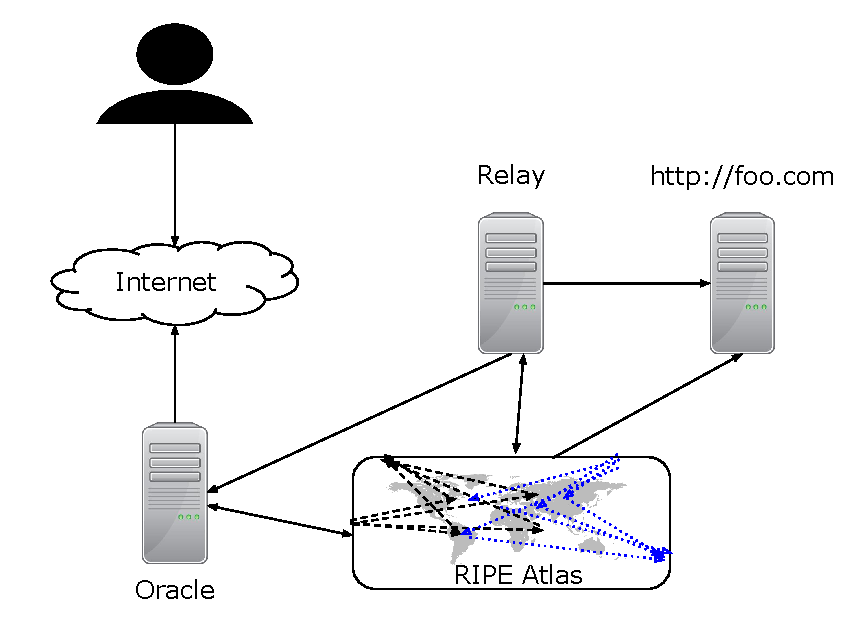
\includegraphics[width=.5\textwidth]{architecture}
\caption{RANSOM architecture.}
\label{fig:arch}
\end{figure}

\subsection{Goals}
Here we highlight the main goals of RANSOM, as well as challenges that are out 
of the scope of this work.

{\bf Foreign Country Avoidance.}  The primary goal of RANSOM is to avoid a given
 country when accessing web content.  RANSOM should provide clients a way to 
route around a specified country, while still being able to access the desired 
domain.

{\bf Usability.} RANSOM should be designed in a way that is accessible to and 
easy to use by clients around the world.  It should require as little effort by 
the client as possible.

{\bf Scalability.}  This country avoidance system should be able to scale to 
large numbers of users.  Therefore, RANSOM should be able to handle the addition
 of relays, as well as be cost-effective in terms of resources required.

{\bf Non-goals.}  There are some challenges that RANSOM does not attempt to 
solve.  The system does not address the notion of anonymity; it routes are 
countries (for reasons such as avoiding mass surveillance), but it does not 
attempt to keep users anonymous.  

Additionally, RANSOM does not solve the problem of domestic surveillance (for 
example, a client in the United States attempting to avoid surveillance by the 
United States).  This is a challenging problem, and asks for future research, 
but this is out of the scope of our work.

\subsection{Calculating Paths}
Given a set of relays that function as proxy servers, it is challenging to 
measure the necessary country-level paths that will allow the system to specify 
which proxy to use for a given domain.  Here we explain which paths we measure, 
and how and where they are measured.  All of the paths are measured using {\tt 
traceroute}, which is then mapped to the country level using the same methods as 
described in Section \ref{datasets} and shown in Figure 
\ref{fig:analysis_pipeline}.

{\bf Client to Relay Paths.}

{\bf Relay to Client Paths.}

{\bf Relay to Server Paths.}

{\bf Client to Server Paths.}

\annie{Discuss re-computation (and include how many country-level paths change per hour/per 2 hours on average, selection of servers/domains, justify argument against traffic analysis because we have 3/4 paths}

\subsection{Multiplexing Between Relays}

\annie{Discuss .pac file and characteristics and generation and re-generation}

\subsection{Adding and Removing Relays}

{\bf Adding Relays.}

{\bf Removing Relays.}

\subsection{Additional Features}

{\bf Privacy-preserving features at proxy.}

{\bf Load balancing and congestion control.}

{\bf Optimized performance.}
